\section{軟弱地面歩行におけるシミュレーション結果}
\label{sec:sim_results}

本節では，前節までで述べたシミュレーション条件に基づき実施した軟弱地面歩行実験の結果について述べる．本節では結果の事実関係のみを整理し，結果に対する解釈や考察については次節で行う．

\subsection{評価した床条件の概要}
\label{subsec:sim_result_conditions}

シミュレーションでは，床の物理特性としてばね定数およびダンパー定数を変更した計4種類の条件を設定し，従来の剛体床を前提とした歩行制御手法を適用した．Case1 および Case2 は高反発ウレタンを模擬した床条件，Case3 は日常的に緩衝材として用いられるスポンジを模擬した床条件，Case4 はシミュレーション上で設定した制御限界付近の床条件である．以下では，各床条件において観測された歩行挙動について述べる．

\subsection{歩行挙動の概要}
\label{subsec:sim_result_overview}

各床条件における歩行挙動を比較した結果，床の剛性および沈み込み特性の違いに応じて，転倒が発生する歩行フェーズおよび挙動の様相が大きく異なることが確認された．高反発ウレタンを模擬した Case1 および Case2 では，床沈み込みが生じた場合でも歩行は継続可能であった．一方で，緩衝材スポンジを模擬した Case3 では，両脚支持期において急激な姿勢変化が発生し，片脚支持期へ移行する前に転倒に至った．また，任意に設定したパラメータである Case4 では，沈み込み中は歩行を維持できたものの，両脚支持期から片脚支持期へ移行した瞬間に転倒が発生した．

\subsection{高・低反発ウレタン床（Case1，Case2）における結果}
\label{subsec:sim_result_urethane}

高・低反発ウレタンを模擬した Case1 および Case2 では，床沈み込みは発生するものの沈み込み量は比較的小さく，従来制御手法においても歩行を継続することが可能であった．沈み込みが生じた直後には，ZMP が一時的に沈み込んだ足裏の外側側面方向へ移動する挙動が確認されたが，その後 ZMP は支持脚足裏内へ戻り，姿勢は安定した．これらの条件では，両脚支持期から片脚支持期への遷移においても転倒には至らず，歩行は最後まで維持された．

\begin{figure}[htbp]
  \centering
  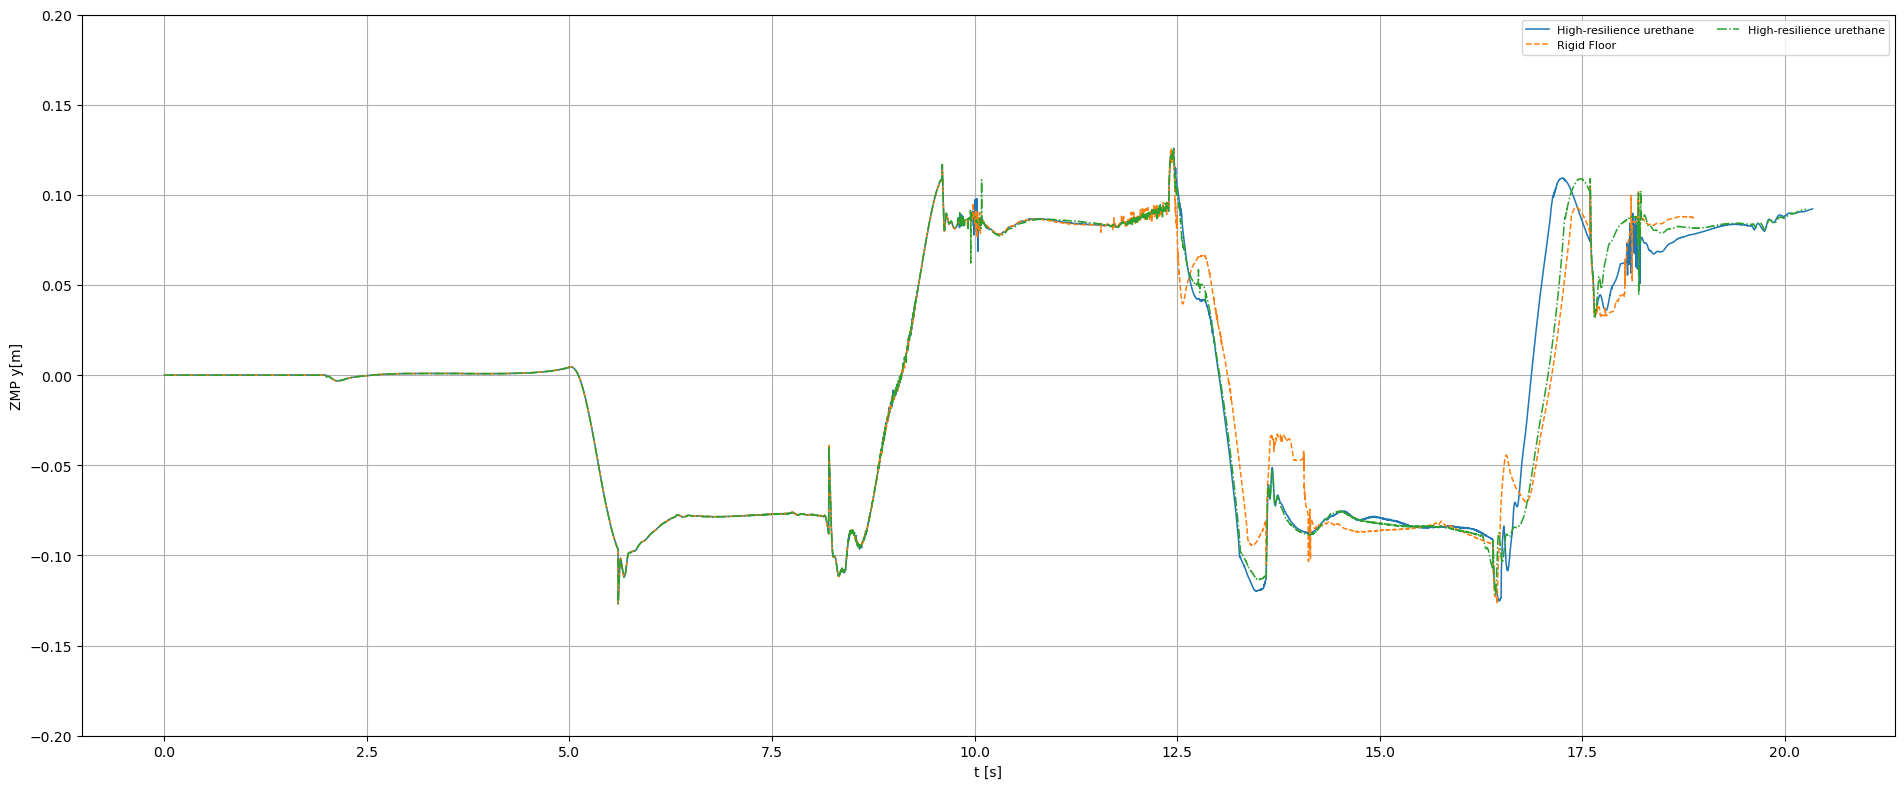
\includegraphics[width=0.9\linewidth]{images/uretan_zmp.png}
  \caption{高・低反発ウレタン床におけるZMP軌道}
  \label{fig:uretan_zmp}
\end{figure}

\subsection{緩衝材スポンジ床（Case3）における結果}
\label{subsec:sim_result_sponge}

緩衝材として一般的に用いられるスポンジを模擬した Case3 では，床の剛性が低いため，接地直後に急激な沈み込みが発生した．この沈み込みに伴い，ロボットの姿勢が両脚支持期において急激に変化し，ZMP が支持脚足裏の外側側面方向へ大きく移動した．その結果，ZMP が支持脚足裏の支持領域を大きく逸脱し，片脚支持期へ移行する前に姿勢を回復できないまま転倒に至る挙動が確認された．

\subsection{シミュレーション設定床（Case4）における結果}
\label{subsec:sim_result_simulated}

シミュレーション上で設定した床条件である Case4 では，床沈み込み中に ZMP が支持脚足裏の外側側面方向へ移動する挙動が確認されたものの，沈み込み中に転倒に至ることはなかった．しかしながら，両脚支持期から片脚支持期へ移行した瞬間に，ロボットは支持脚とは反対側の遊脚方向へ傾き始め，次の接地動作に入る前に転倒するケースが確認された．この条件では，沈み込みそのものよりも，歩行フェーズ遷移時の挙動が転倒に強く関与していることが観測された．

以上の結果から，軟弱地面歩行においては床沈み込みの大きさや速度だけでなく，転倒が発生する歩行フェーズが床条件によって異なることが明らかとなった．次節では，これらの結果に基づき，特に Case3 および Case4 において歩行が不安定化した要因について力学的観点から考察を行う．
